\documentclass{article}

\usepackage[utf8]{inputenc} % accents
\usepackage[T1]{fontenc}      % caractères français
\usepackage{geometry}         % marges
\usepackage[francais]{babel}  % langue
\usepackage{graphicx}         % images
\usepackage{verbatim}

\title{Rapport Projet Approche Objet}
\author{Alexandre Casanova-Franger\\
        \and
        Gauthier Lamarque\\
        \and
        Zakaria Mallouky\\
        \and
        Lucas Vivas\\
        }

\begin{document}
  \maketitle
  \section{Bilan}
  \paragraph{}
  Le jeu du Labyrinthe est fonctionnel. Dans un premier temps, nous générons un
  labyrinthe parfait, et ensuite nous ajoutons un grand nombre d'arêtes au
  graphe pour que nous puissions semer les méchants et rejoindre la porte de
  sortie sans encombre. Le joueur débute le niveau en haut à gauche du
  labyrinthe, et la porte se situe à la case la plus éloignée de la position de
  départ (souvent en bas à droite logiquement). Les méchants, dans une première
  version, se déplaçaient en même temps que le joueur effectuait un déplacement.
  Ensuite, nous avons implémenté des threads afin que les méchants se déplacent
  indépendamment du joueur. Nous avons disposé aléatoirement sur le labyrinthe
  des bonbons censés rapporter au joueur des "points" en focntion du type de
  bonbon ramassé. Nous n'avons pas encore, pour l'heure, terminé ce système de
  points.\\
  De plus, nous avons determiné trois niveaux de difficulté, et le changement
  entre ces trois niveaux est la vitesse de déplacement des méchants.

  \paragraph{}
  Pour améliorer notre projet en terme de fonctionnalités, nous aurions pu, bien
  entendu ajouter plein d'autres bonus, comme une série de niveaux où la
  difficulté augmente graduellement, grâce notamment à la vitesse de déplacement
  des méchants, ou au nombre d'arêtes ajoutées dans le graphe (donc le
  labyrinthe). Le système de points et de bonbons pourrait être amélioré. Comme
  vous l'avez rappelé en TD, tout cela n'est que du "sucre", c'est-à-dire des
  éléments bonus.\\
  Du point de vue de l'architecture, nos classes sont vraisemblablement trop
  couplées. Pour remédier à ce problème, plusieurs options s'offrent à nous:
  \begin{itemize}
    \item créer des contrôleurs intermédiaires liant un élement du modèle à
    l'élément de la vue correspondant,
    \item faire communiquer le modèle et la vue par le biais d'une fonction
    refresh() qui redessinerai les éléments modifiés dans le modèle.
  \end{itemize}
  Enfin, certaines fonctions ou attributs ne sont peut être pas placé de façon
  optimale au sien de notre code. Il se peut dès lors que certains appels
  intermédiaires soit superflus, que la cohésion de nos classes faiblissent.

  \section{Design patterns}
  \paragraph{}
  Pour réaliser ce projet, nous avons organisé notre code selon l'architecture
  MVC. Nous avons autant que nous le pouvions respecter le fait que les
  communications entre le modèle et la vue passent forcément par le contrôleur.
  Les entrées clavier sont captées par le contrôleur.\\
  On a utilisé le design pattern Singleton pour le modèle, la vue, le
  contrôleur,la classe Player, la classe Graph, la classe Door. Plus
  généralement, tous les éléments qui sont censés n'apparaître qu'une fois ont
  été codés avec le design pattern Singleton.\\
  Toujours dans l'optique d'utiliser des design patterns pertinents, nous avons
  choisi d'implémenter le design pattern Observer pour ce qui concerne les
  personnages méchants (BadGuy dans le code) afin que lorsque le joueur effectue
  un mouvement, tous les méchants soient avertis de la nouvelle position du
  joueur pour que ceux-ci re-calculent la distance qui les sépare du joueur avec
  l'algorithme de Manhattan.\\
  Enfin, nous avons fait le choix d'utiliser le design pattern Factory pour ce
  qui concerne les bonbons. Comme il y a plusieurs types de bonbons différents,
  la Factory les génére de manière aléatoire.

  \section{Réalisations}
  \paragraph{}
  Tout au long du projet, chaque membre du groupe a plus ou moins touché à tout
  le code, il serait donc presque impossible de dire exactement qui a fait
  quelle fonction. Toutefois, nous allons décrire ci-dessous qui s'est occupé
  de quelle fonctionnalité en général.

  \paragraph{}
  Lucas et Alexandre ont réalisé la première ébauche du labyrinthe en
  construisant le squelette du modèle et du graphe ainsi que la vue qui
  permettait d'afficher tout cela. Par la suite, Gauthier et Zakaria ont décidé
  de remanier la classe Graph, car celle-ci comportait des éléments redondants
  et inutiles. Pour la suite, Zakaria et Gauthier se sont occupés d'implémenter
  le mouvement du joueur ainsi que de la gestion des entrées clavier.\\
  Lucas et Alexandre ont par la suite intégré les éléments manquants du jeu,
  c'est-à-dire les méchants et la porte de sortie, tant au niveau du
  modèle qu'au niveau de la vue.\\
  Gauthier s'est occupé de corriger les mouvements des méchants, pendant
  qu'Alexandre leur appliquait le design pattern Observer, et enfin Zakaria a
  implémenté des threads afin que les méchants bougent indépendamment du joueur.
  Enfin, Lucas et Gauthier se sont occupés des commentaires permettant de
  générer la Javadoc, et Gauthier (pour l'instant) s'est occupé de la rédaction
  de ce rapport.

  \section{Architecture du code}
  \paragraph{}
  Ci-dessous vous trouverez un diagramme représentant l'héritage de nos classes.
  Il ne représente pas les liens de composition mais on peut néanmoins voir les
  attributs de chaque classe.\\

  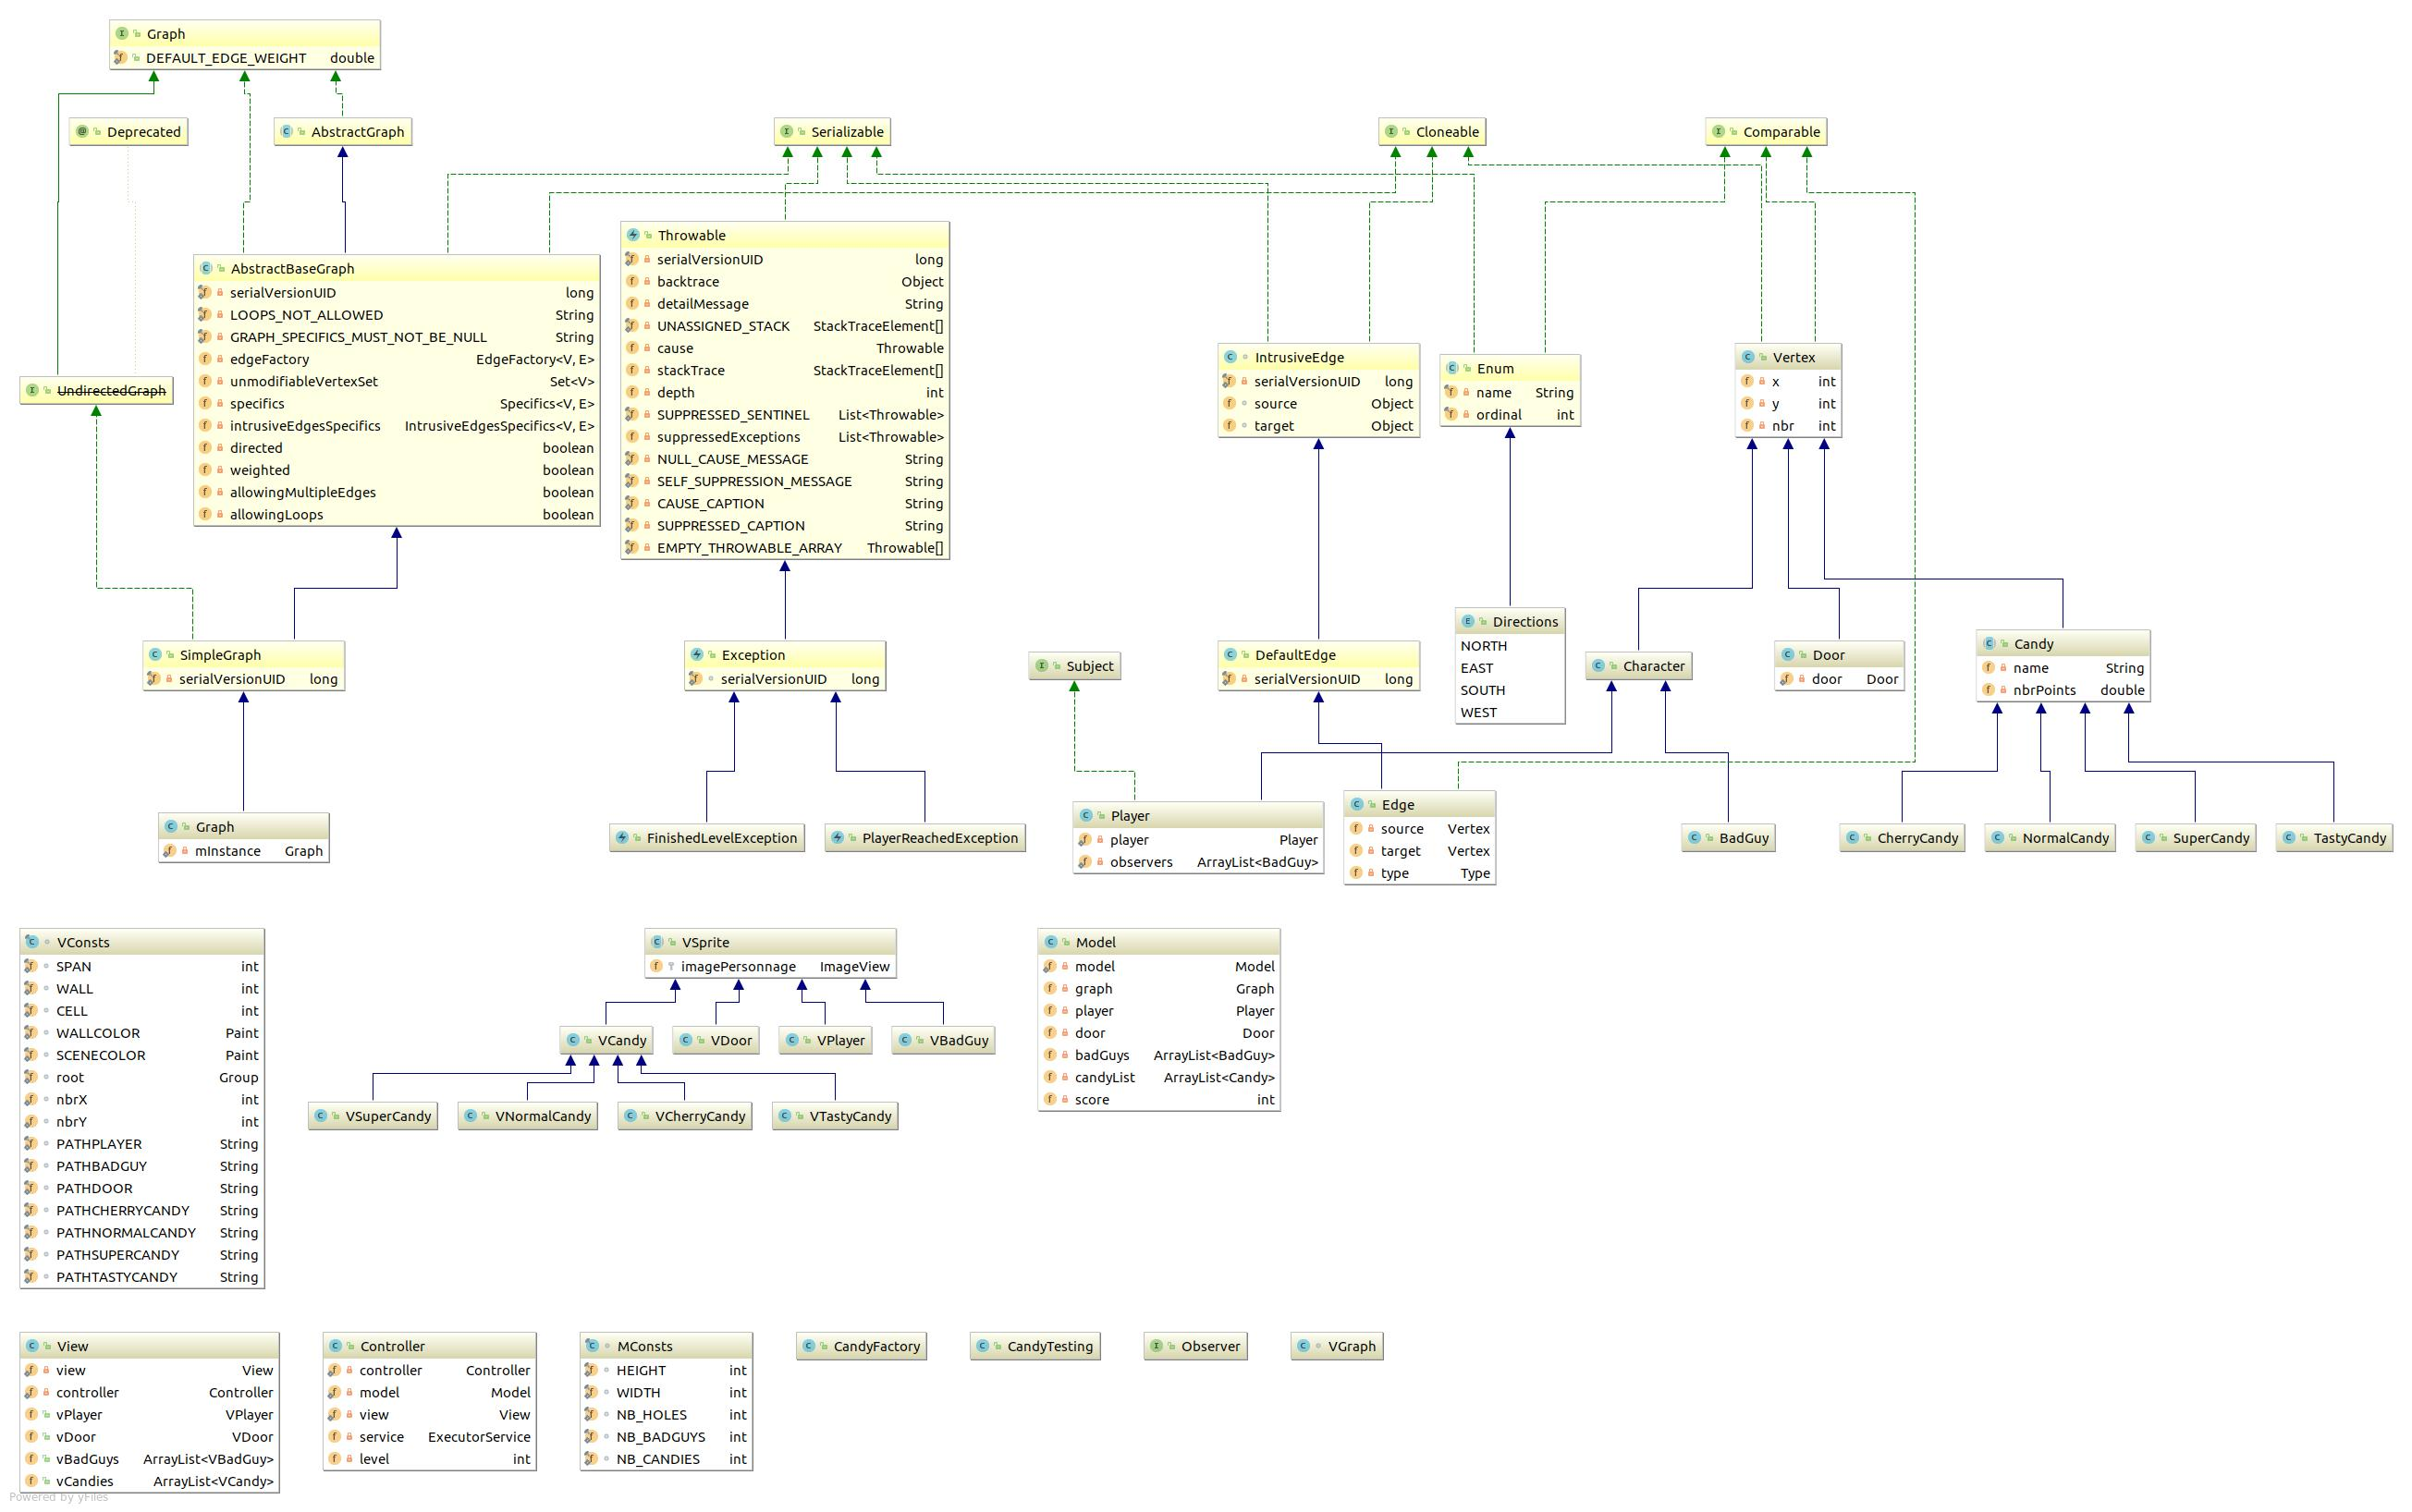
\includegraphics[width=17cm]{Controller2.jpg}



\end{document}
